\chapter{Introduction}
\label{sec:intro}
\section{Scope}
\begin{figure}
\centering
\begin{tabular}{@{}c@{}c@{}}
	 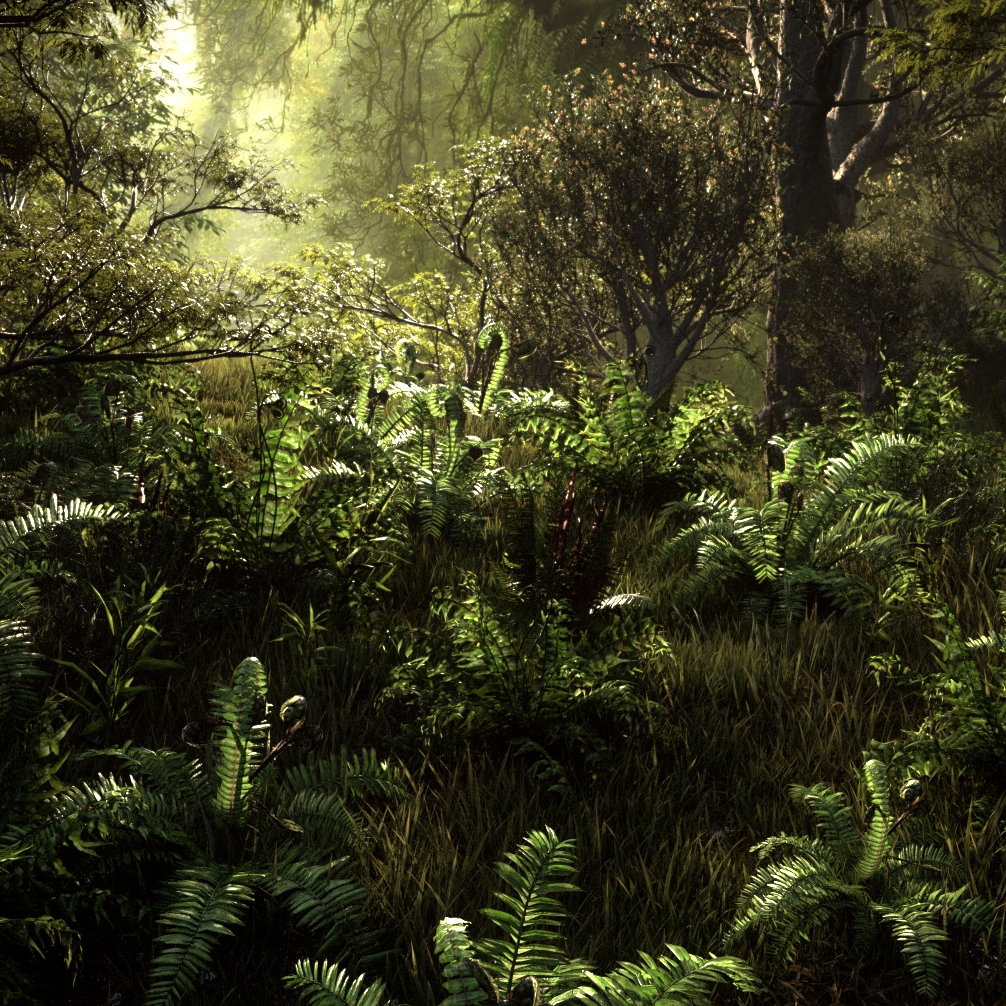
\includegraphics[width=0.5\textwidth]{figures/forest-maya-crop.jpg} & 	 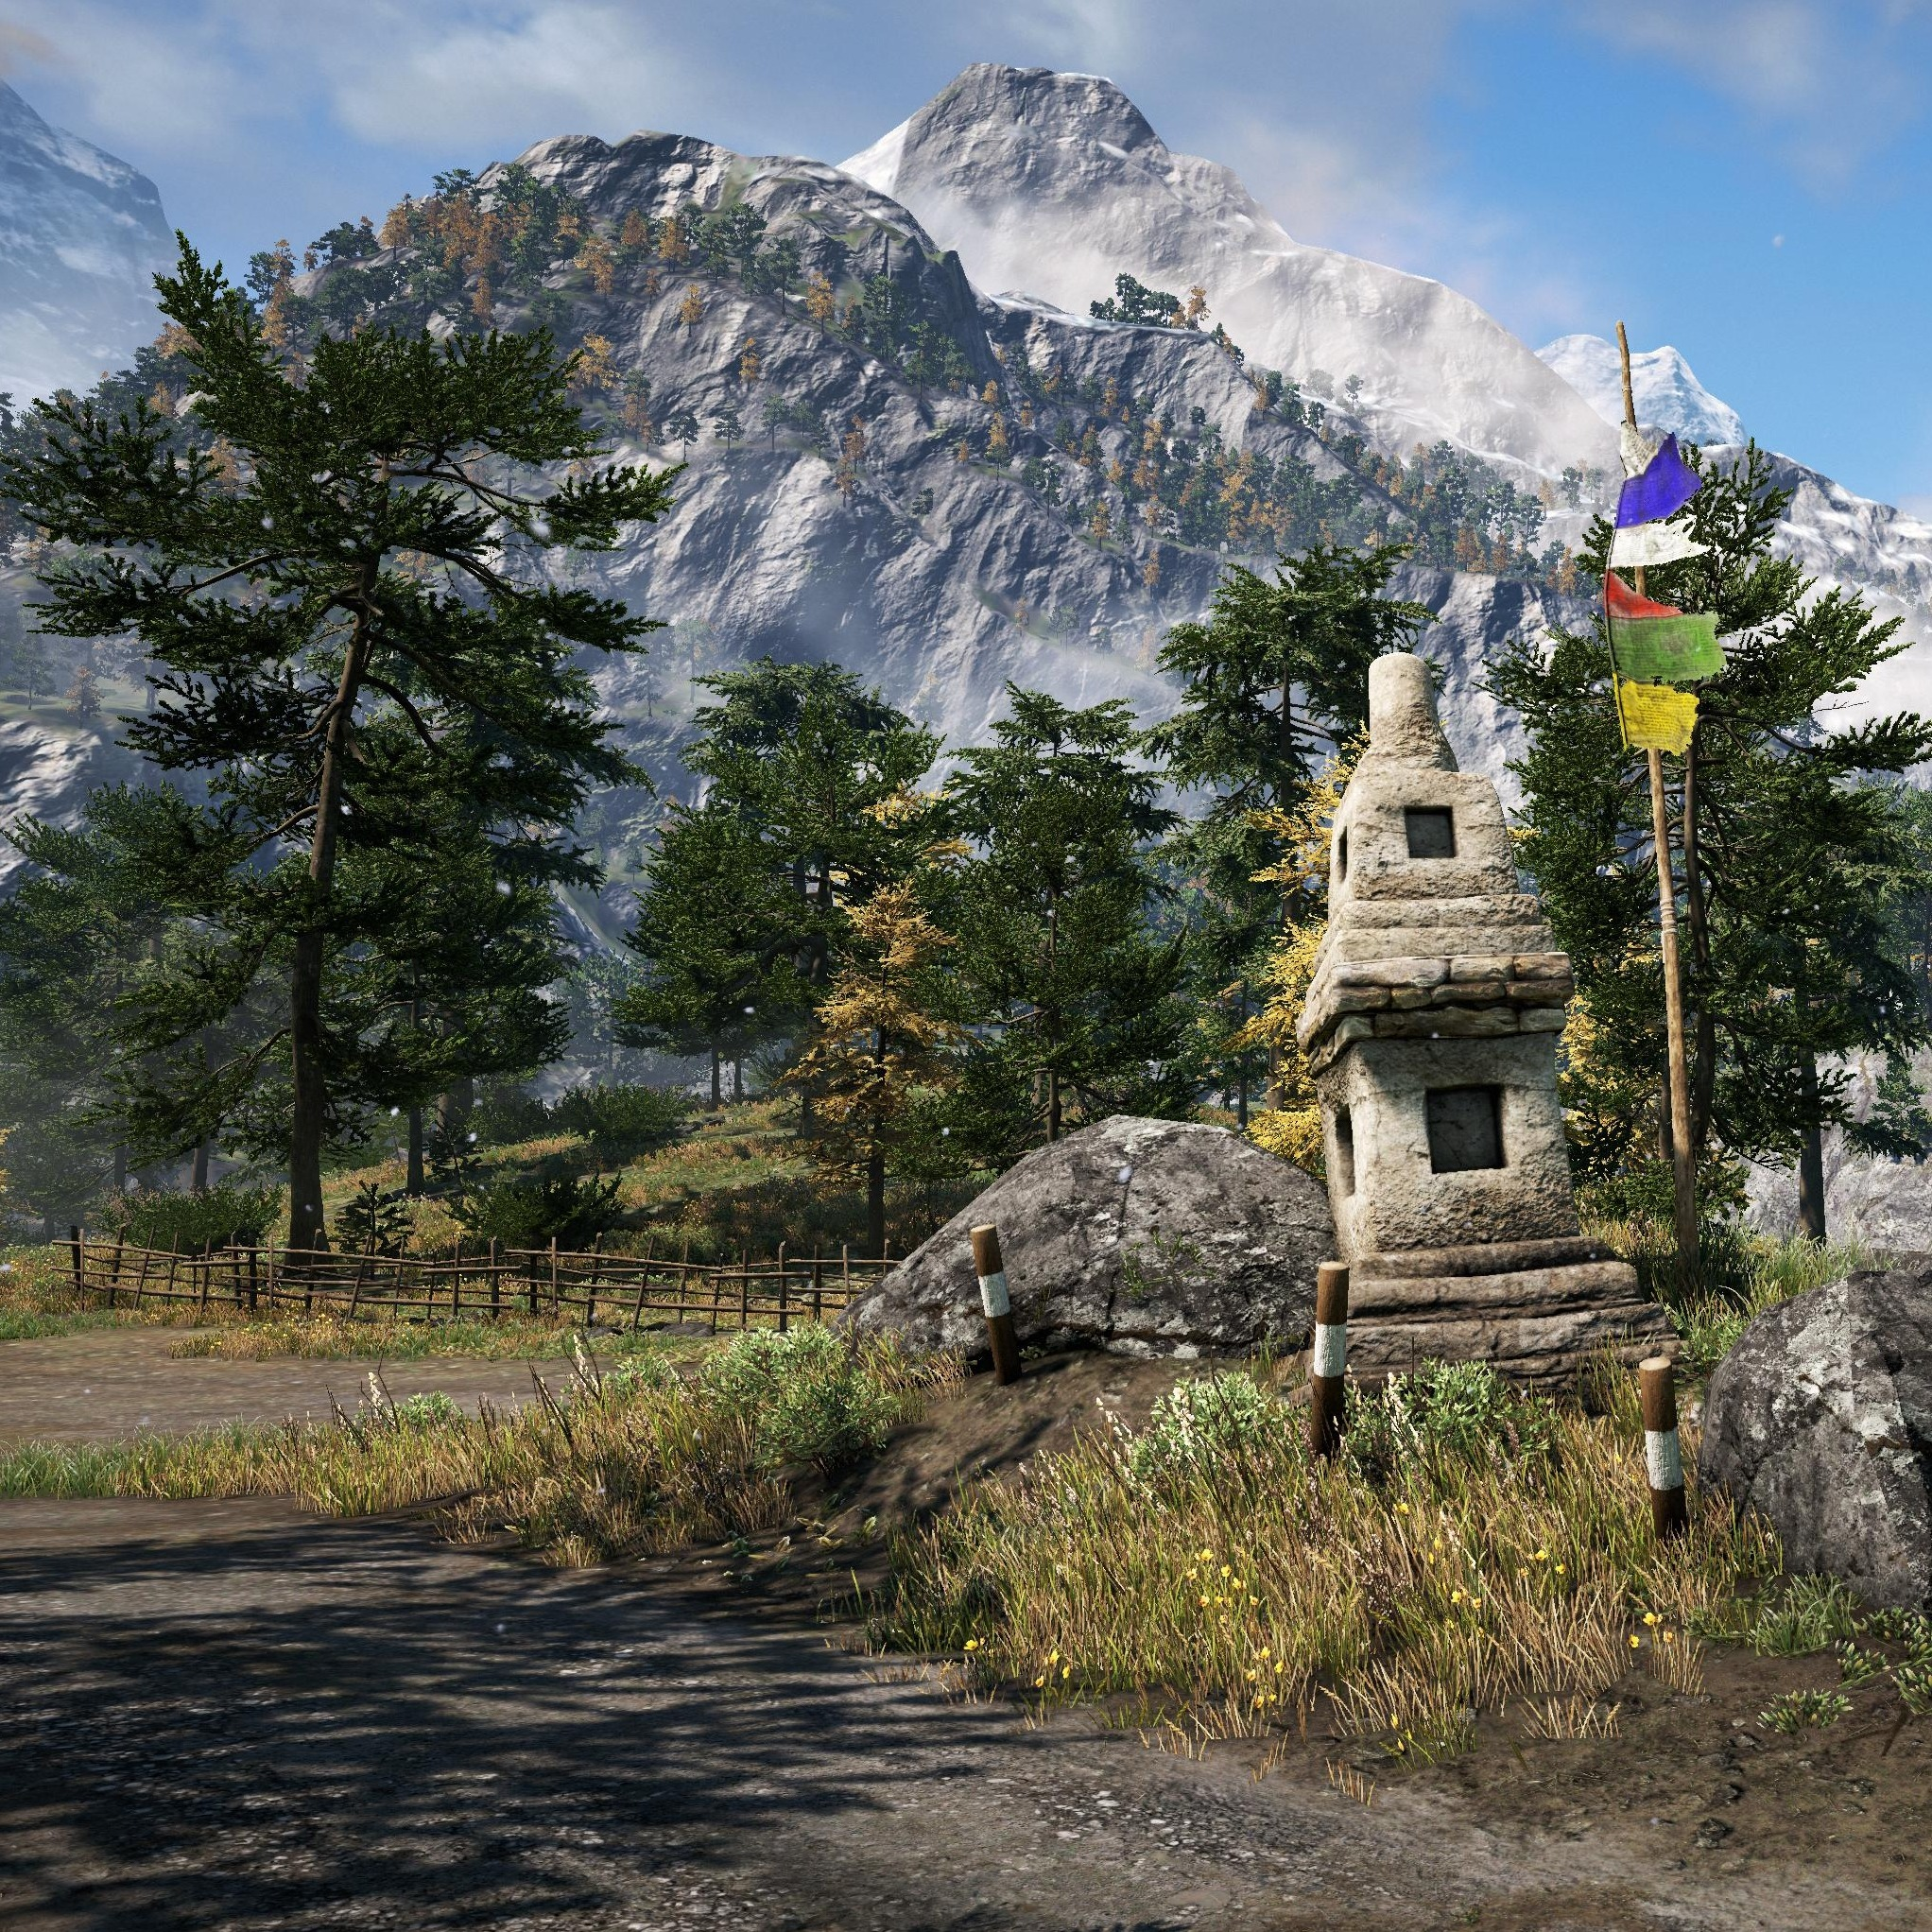
\includegraphics[width=0.5\textwidth]{figures/far-cry-4-crop.jpg} \\
\end{tabular}
\caption{Some examples of interactive and non-interactive photorealistic rendering. Left, rendering of a forest obtained in Maya (courtesy Greg Zdunek). Right, real time rendering in \emph{Far Cry 4} (courtesy Ubisoft). } 
\label{fig:main_examples}
\end{figure}

The main goal of this thesis is to describe new techniques to bring movie production quality rendering into interactive applications.  The goal is to achieve photorealistic appearance as close as possible to the real world, while retaining the possibility for the user to interact with the simulation. 
Interactive realistic rendering applications are relevant in many fields, including
\begin{itemize}
\item 3D digital modeling and 3D printing,
\item Product development and visualization
\item Digital prototyping
\item Computer games and animation
\end{itemize}
In recent years, many advances have been made to achieve photorealistic quality in the interactive applications listed above, often achieving results that are perceptually and remarkably closer to slower photorealistic rendering techniques (see Figure~\ref{fig:main_examples}). This thesis contributes with various techniques, exploring the area between interactive and real time rendering techniques (e.g.\ rasterization and interactive ray tracing) and photorealistic rendering techniques (e.g.\ path tracing, hierarchical point cloud methods), with the goal of applying photorealistic appearance models (BRDFs and BSSRDFs, both analytical and measured). As most modern rendering techniques, we exploit the high throughput of graphics processing units (GPUs). Our contributions exploit both the long standing GPU hardware rasterization pipeline, but also focus on applications of the currently expanding field of interactive ray tracing. 

\section{Motivation}
\label{sec:motivation}
\begin{figure}
\centering
\begin{tabular}{@{}c@{}c@{}c@{}c@{}c@{}}
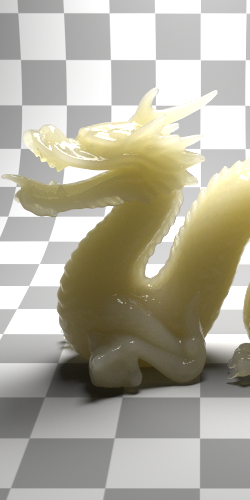
\includegraphics[width=0.2\textwidth]{figures/thesis_pt}& 	 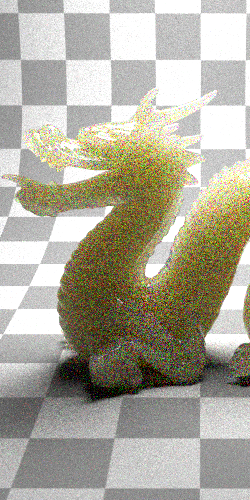
\includegraphics[width=0.2\textwidth]{figures/thesis_pt_unconverged} &
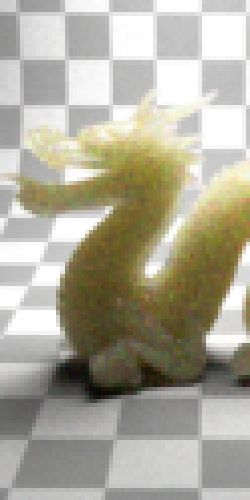
\includegraphics[width=0.2\textwidth]{figures/thesis_pt_unconverged2}& 	 	 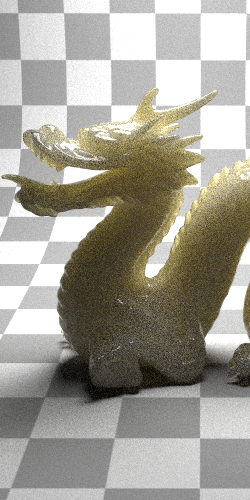
\includegraphics[width=0.2\textwidth]{figures/thesis_pt_sd}& 	 	 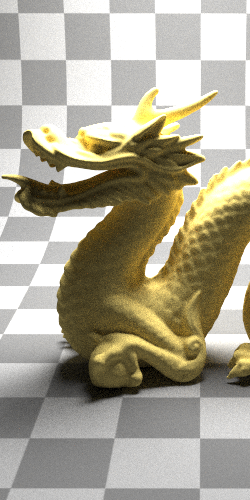
\includegraphics[width=0.2\textwidth]{figures/thesis_pt_lambertian} \\
\end{tabular}
\caption{Comparing different preview techniques. From left to right: converged image, noisy unconverged image, downsampled image, different physical model, diffuse appearance. All images took 120 seconds to render on a GPU ray tracer. Converged result took 4 hours.} 
\label{fig:comparison_convergence}
\end{figure}

From the beginning of computer graphics, researchers have been striving to synthesize more and more realistic images. Nowadays, for still images and carefully crafted scenes, it is almost impossible to distinguish a synthetic image from an actual photograph. To achieve these photorealistic images, a great amount of hours must be spent in modeling or acquiring the 3D geometry, and choosing or measuring the correct materials. Finally, some time must be spent rendering the image, that can take up to several hours. In the rendering part, the more advanced the physical model used, the higher the rendering time. This high rendering time can cause production bottlenecks, e.g. when some artistic tweaking is needed to achieve a specific style or artistic constraint. Once the tweaks are performed, the whole rendering needs to be redone in order to see the influence of the tweak on the final result, wasting precious production time. 

To mitigate this problem, many applications display a preview of the final rendering result. Depending on the application the technique can be different (see Figure~\ref{fig:comparison_convergence}), like displaying a noisy result, a spatially downsampled one, or simply switching to a simpler rendering model. All these techniques come with different trade offs, advantages and disadvantages. In general, these preview techniques trade physical accuracy in exchange to getting rid of noise. 

Given these problems, when immediate feedback is important, there is a need in the industry for clever techniques that exploit the main two rendering constraints, namely time and accuracy. We classify and visualize various applications according to these constraints in Figure~\ref{fig:main_diagram}. The first constraint, allowed rendering time, ranges from a few milliseconds per frame in a real-time environment (e.g.\ games or virtual reality), to some fractions of a second (e.g.\ 3D printing preview) up to some minutes or hours (e.g\ a frame in movie production environment). The second constraint we mentioned is accuracy, i.e. the accuracy in modeling the physical process behind the rendering. In some applications, the accuracy is  limited. For example, in a video game, it is more important to obtain a fast result that feels physically correct rather than a physically accurate result. In some other applications, the requirements are stricter: think architectural light simulation, where architects need to know precisely how the light reacts to different surfaces to see the overall illumination of the environment. 

We now discuss three more detailed use cases in which there is a demand for improvements in photorealistic rendering techniques, visualized in Figure~\ref{fig:applications}. These cases are not meant to be comprehensive of all applications in which interactive photorealistic rendering techniques are needed. However, they provide insights on possible industrial applications of the various contributions within this thesis.

\begin{figure}
\centering
	 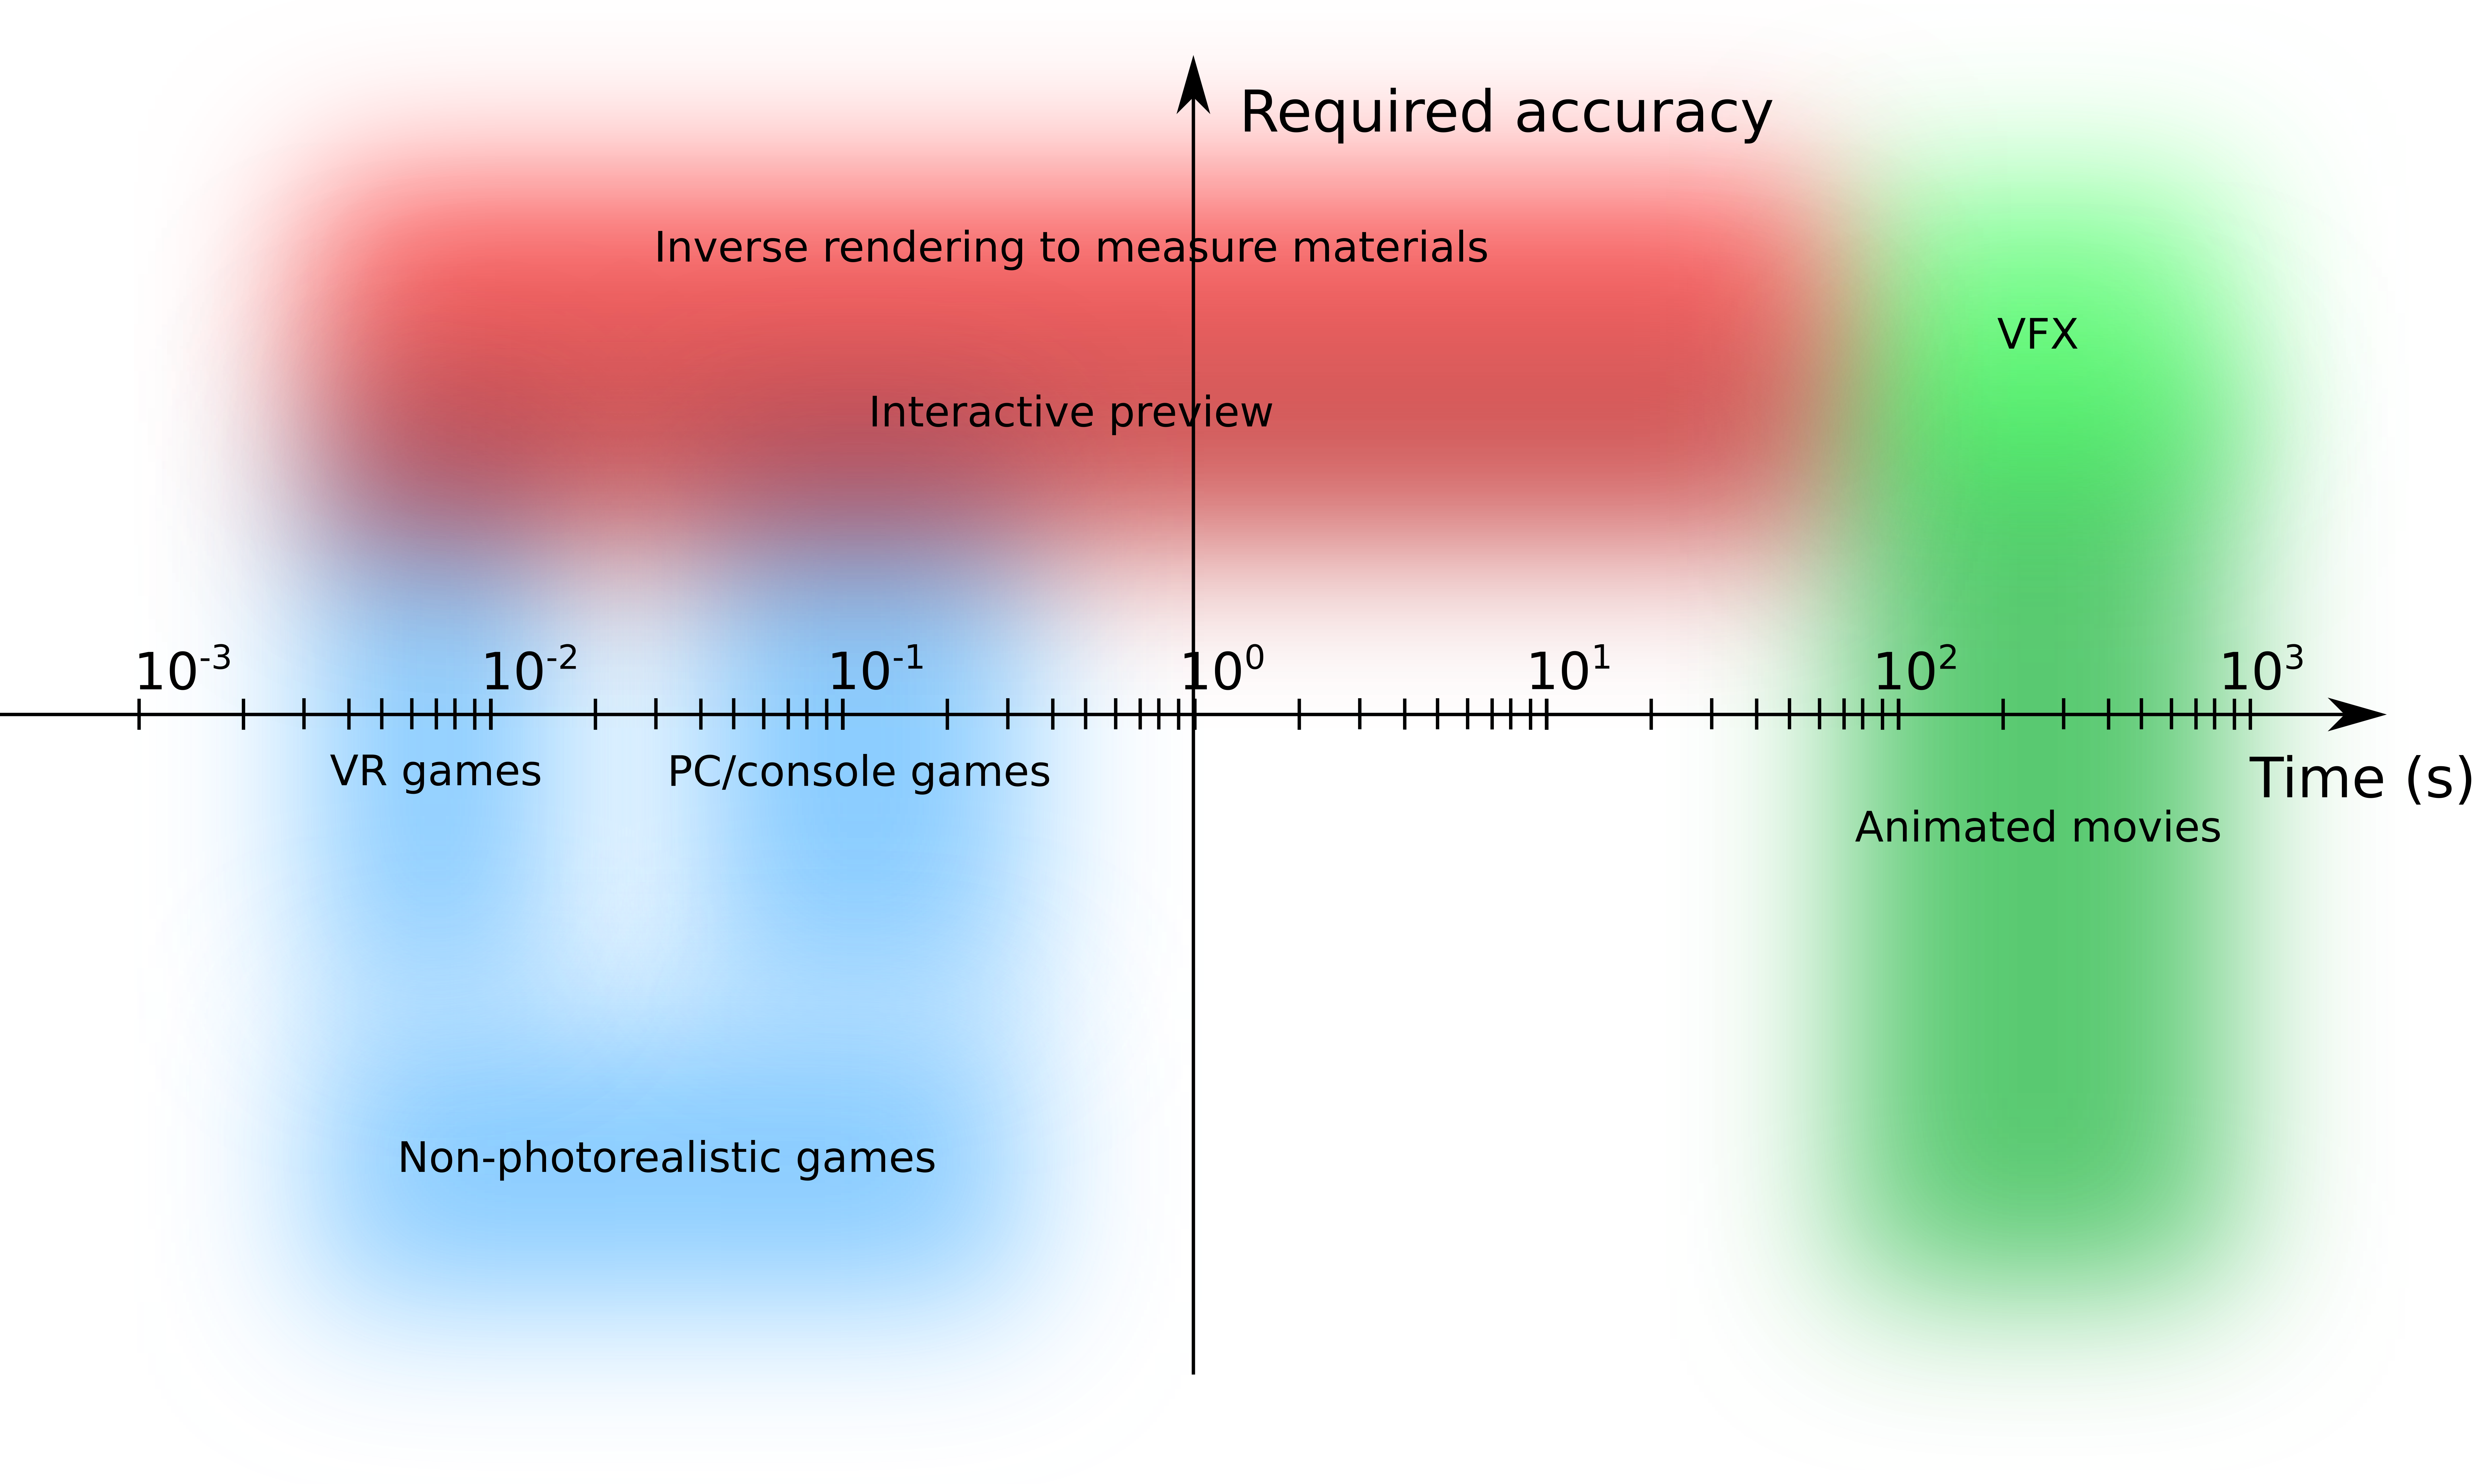
\includegraphics[width=\textwidth]{figures/photorealistic_diagram.png}  \\
\caption{Visualizing the time-accuracy graph, showing the  different application fields.} 
\label{fig:main_diagram}
\end{figure}

\begin{figure}
\centering
\begin{tabular}{@{}c@{}c@{}c@{}}
	 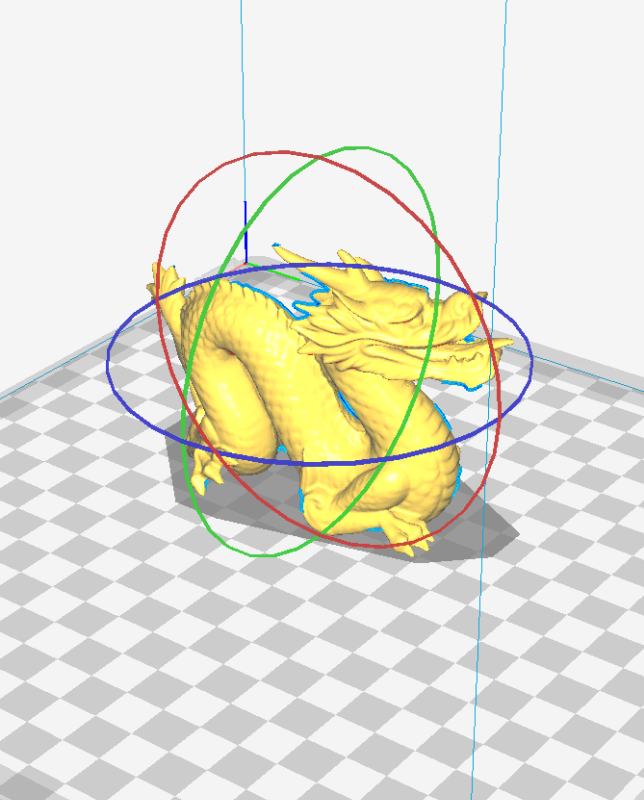
\includegraphics[width=0.33\textwidth]{figures/3dprinting_preview_crop} & 	 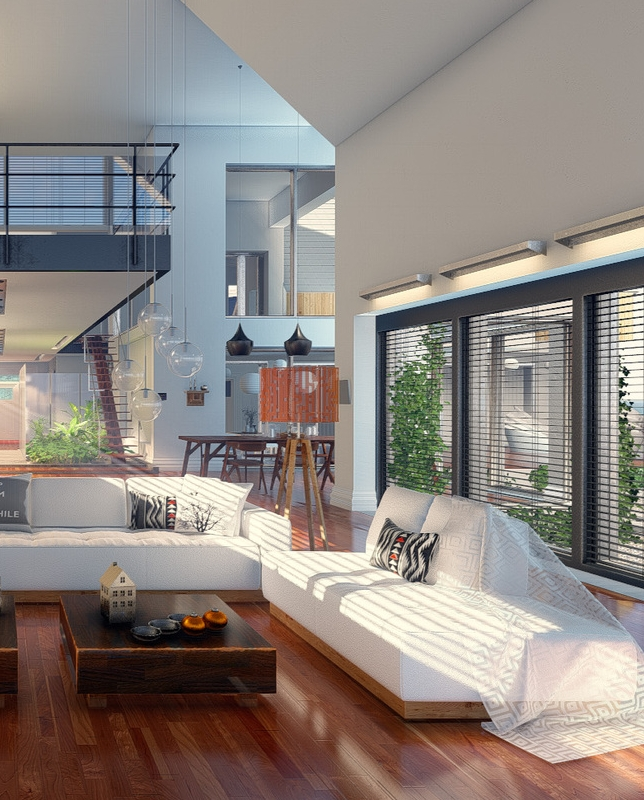
\includegraphics[width=0.33\textwidth]{figures/lumion-crop.jpg} 
& 	 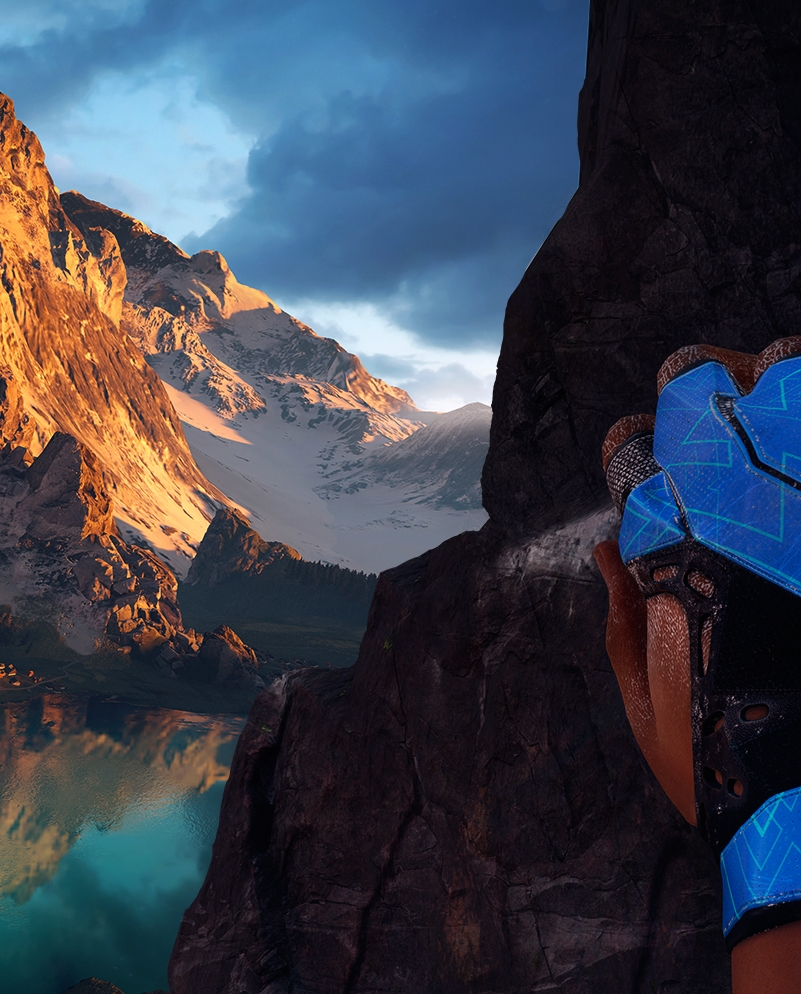
\includegraphics[width=0.33\textwidth]{figures/the-climb-crop.jpg} \\
\end{tabular}
\caption{Applications of photorealistic interactive rendering. Left to right: preview in 3D printing application, architectural visualization (courtesy \emph{Lumion}), virtual reality games (courtesy \emph{The Climb} by \emph{Crytek}).} 
\label{fig:applications}
\end{figure}

\subsection{Digital prototyping and 3D printing}
The first case we discuss applications of interactive photorealistic rendering is digital prototyping, in particular applied to 3D printing. In this application, we want to preview the appearance of a manufactured object. In the particular case of 3D printing, the production process greatly influences the shape and the appearance of the final object. Moreover, the materials used for 3D printing exhibit some particular radiometric properties, that makes them even more challenging to render accurately. 

In this application, the role of photorealistic rendering is dual. Apart from previewing the final result of the 3D printing process, we can actively use photorealistic rendering to predict and measure the radiometric properties of the object. This requires a  specific setup and calibrated scene, in which a picture of the object is taken. Then, lots of different renderings can be made, tweaking the radiometric properties to predict the final appearance of the object. In both these applications, we require a high accuracy in our rendering (see Figure~\ref{fig:main_diagram}). In this case, a noisier or downsampled result can be acceptable, at the price of a certain inaccuracy in measuring the parameters. We will explore this topic in our Contributions~\ref{sec:juice} and~\ref{sec:glass} (see also Section~\ref{sec:definingphoto}).

All these innovations go towards a more strict integration of 3D printing processes and digital image synthesis as a whole (the digital-physical ecosystem). Photorealistic rendering helps reduce the number of iterations necessary to achieve a satisfying printed piece. This translates to reduced printing times for the same quality, and it avoids wasting potentially expensive printing material. Moreover, in a digital production  environment, the validation through rendering enables us to perform quality assurance on the finished pieces, by comparing them with images of previously printed versions of the same piece.

\subsection{Architectural visualization}

Our second case is architectural visualization. In this particular field, architects use interactive visualization tools to show how light propagates through a building at different times of the day. This allows to create buildings that best use natural illumination, minimizing electricity consumption for the building. In this particular application, an important focus is placed on accurately represent materials. Materials used in construction like frosted glass, marble or cloth, are radiometrically complex and hard to render fast and accurately. These materials can be either measured using some sort of apparatus, or matched by an artist so that they represent the appearance and light interaction properties of the original material. Given the complexity of the models and the generally needed artistic tweaking time, we found this field an interesting application field for interactive photorealistic techniques.

Recent efforts have been trying to offer a more interactive experience, in order to show the finished product to project stakeholders. So, architectural visualization is moving towards interactive or real-time visualization, in particular in a virtual reality environment. Furniture giant IKEA is a particular example of this, where they use virtual and augmented reality to show how different pieces of furniture would fit in your own house. Virtual reality pipelines need to maintain the same standard of physically based accuracy as the original simulation, while fitting into extreme time constraints, a handful of milliseconds per frame. In this case, fast techniques that exploit current hardware to achieve photorealistic visualization are even more important.


\subsection{Computer games}

The final application of fast interactive photorealistic techniques we discuss is in computer games. Computer games have the strictest time constraints of all the applications so long presented. For a standard frame in a game, the industry standard is around 16 milliseconds (60 frames per second). In recent year, virtual reality games are starting to become prominent, lowering the standard to 7-11 milliseconds total (90-120 frames per second). Generically, games use triangle based rasterization, so that they can leverage custom hardware on GPUs. 

As games vary for gameplay, environment and style, photorealistic rendering can or cannot be employed in games. Nowadays, a good number of games strive to achieve a photorealistic or quasi-photorealistic look. In games, the focus is on performance and immersiveness, so the simulation does not need to be accurate from a physical standpoint. Actually, sometimes the rendering algorithms are made non realistic on purpose to achieve a specific artistic look. Given the hard time constraints, specific techniques need to be developed to achieve a photorealistic look. These techniques are often tailored to a specific game, and no overall solution for all games exists. This makes it an interesting field to contribute with general scalable physically based techniques, with the ultimate goal to reduce production costs.

\section{Outcome}

\begin{figure}
\centering
\begin{tikzpicture}[      
        every node/.style={anchor=south west,inner sep=0pt},
      ]   
     \node (figmain) at (0,0)
       {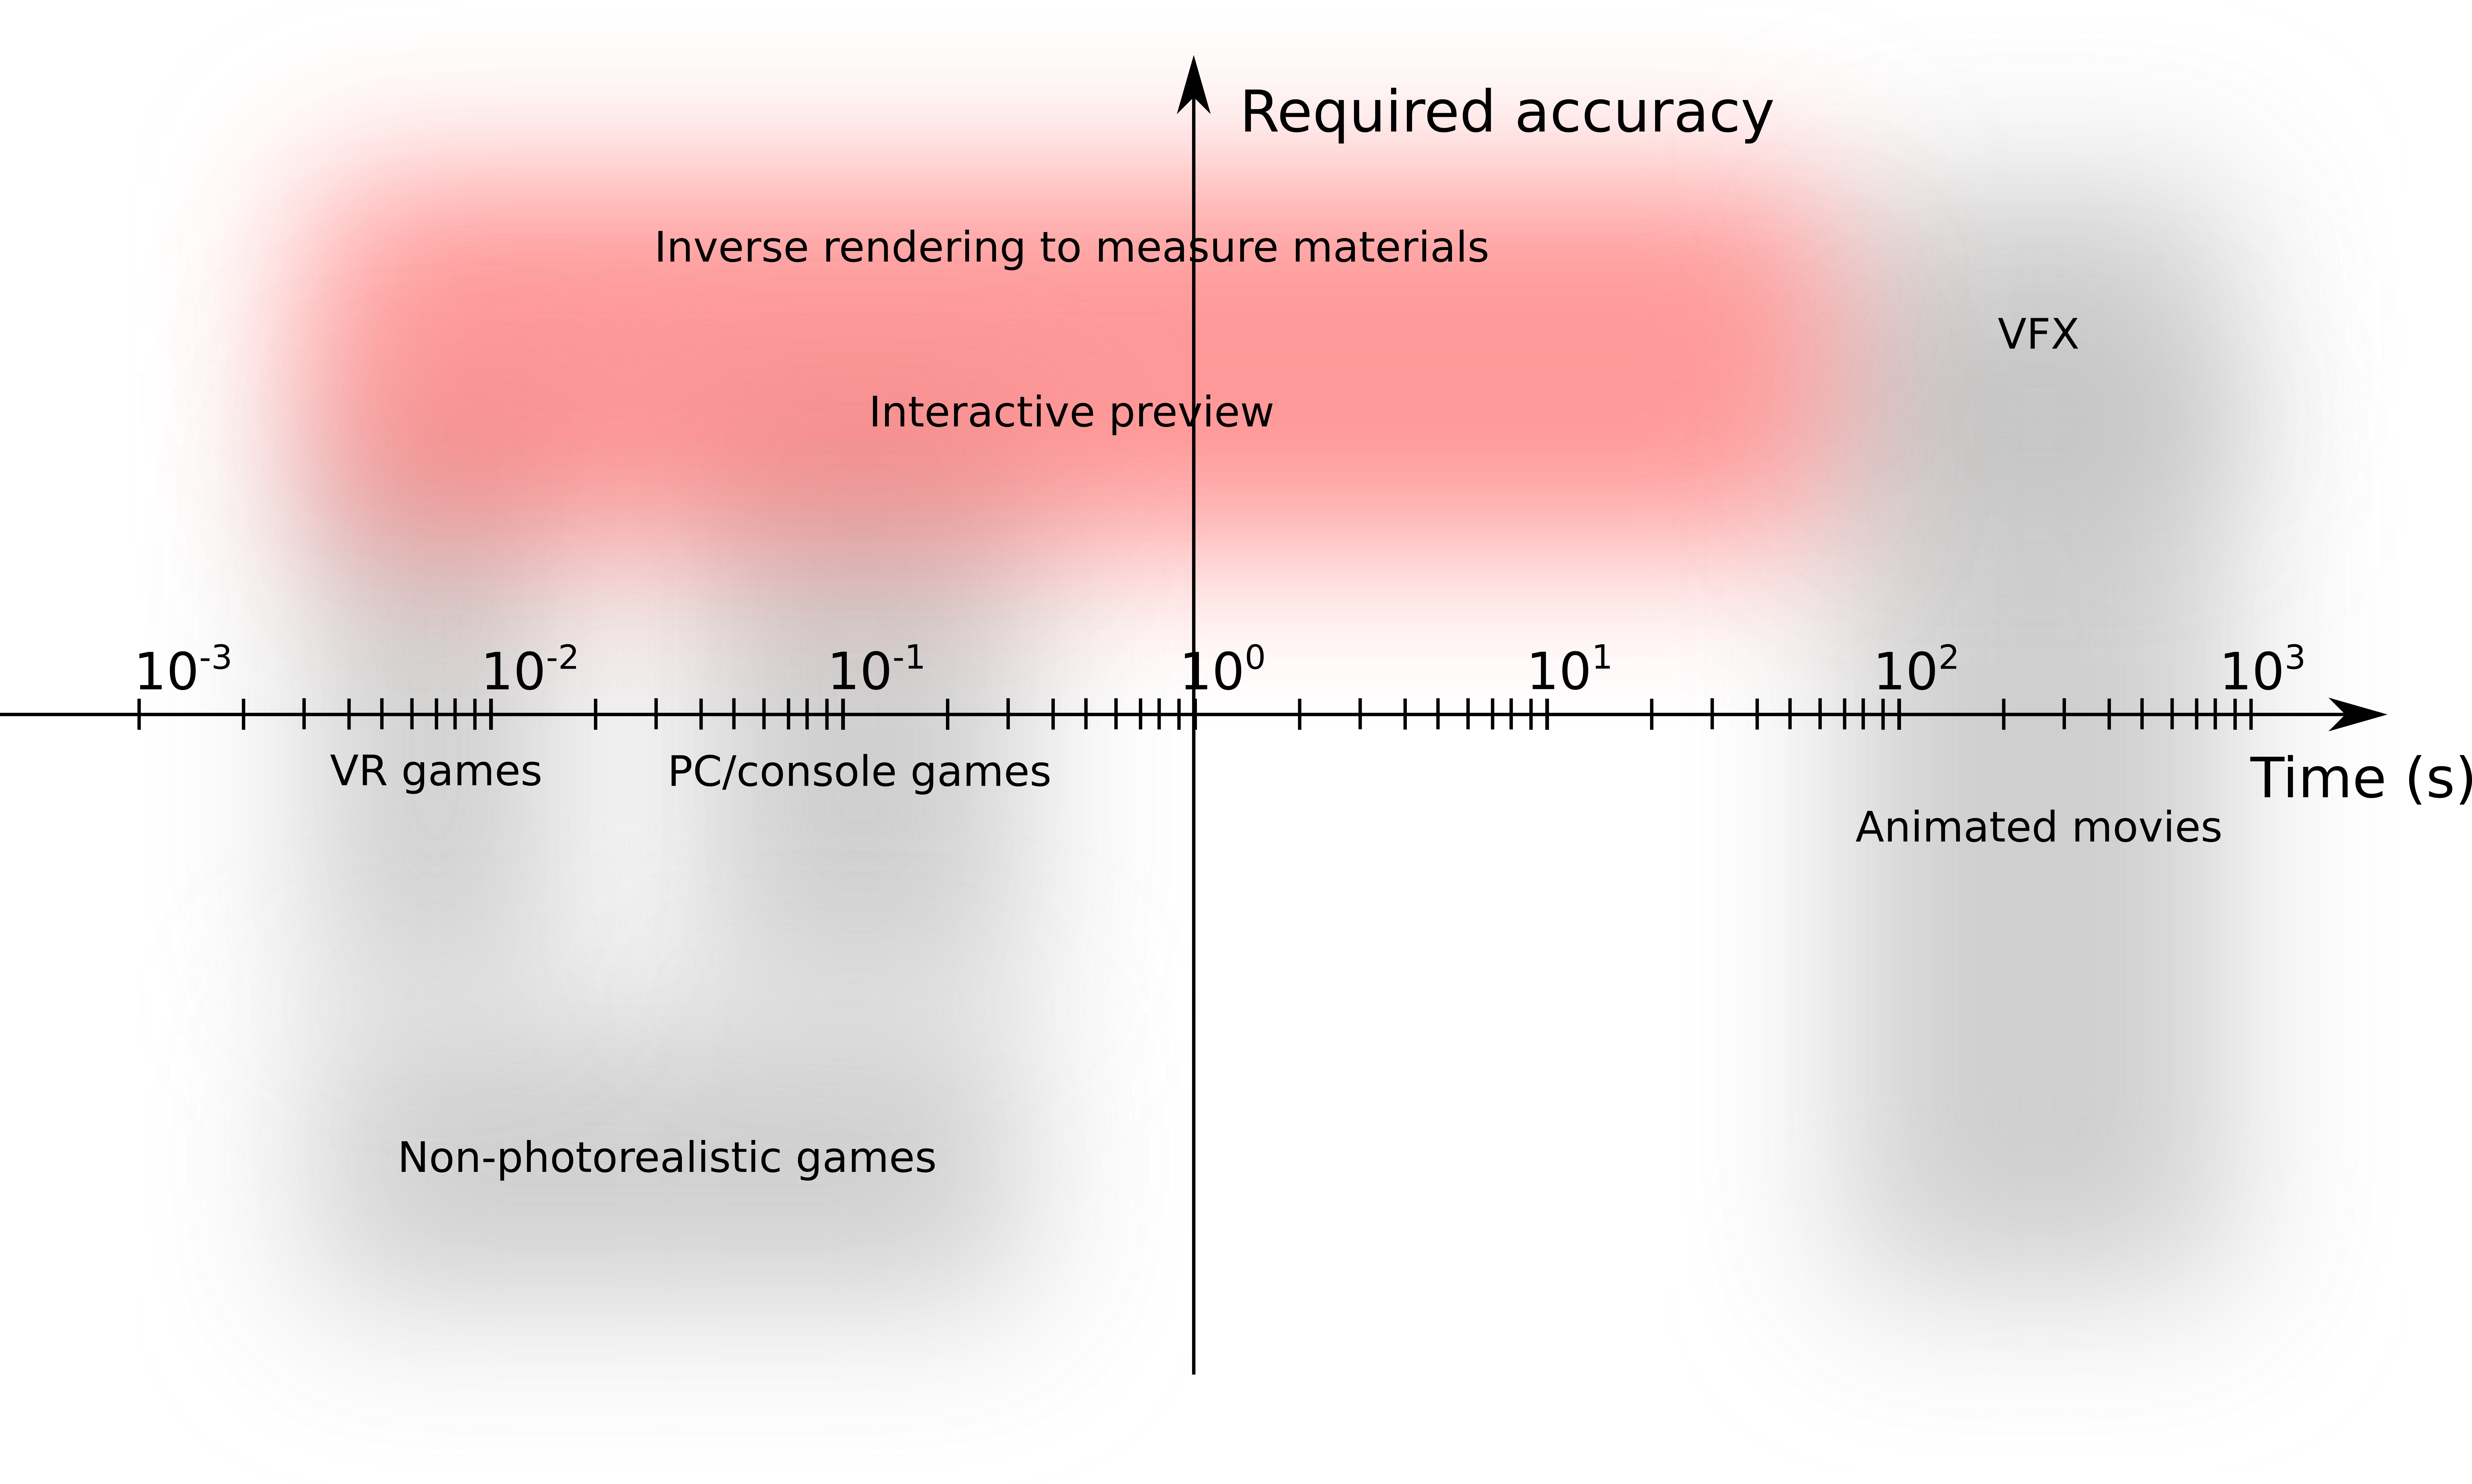
\includegraphics[width=\textwidth]{figures/photorealistic_diagram_bw}};
      \node (fig0) at (0.6\textwidth,0.45\textwidth)
       {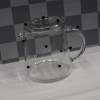
\includegraphics[width=0.15\textwidth]{figures/thumbnails/ao17_reassembly}};
      \node (fig1) at (0.27\textwidth,0.32\textwidth)
       {
\includegraphics[width=0.15\textwidth]{figures/thumbnails/dirsss_tvcj16}};
      \node (fig2) at (0.5\textwidth,0.4\textwidth)
       {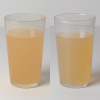
\includegraphics[width=0.15\textwidth]{figures/thumbnails/mam}};
      \node (fig3) at (0.25\textwidth,0.2\textwidth)
       {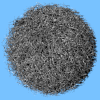
\includegraphics[width=0.15\textwidth]{figures/thumbnails/srt}};
      \node (fig4) at (0.1\textwidth,0.3\textwidth)
       {
\includegraphics[width=0.15\textwidth]{figures/thumbnails/vr_showcase_brdf}};
\node[above = -0.25cm of fig0] {\colorbox{white}{\ref{sec:glass}}};
\node[above = -0.25cm of fig1] {\colorbox{white}{\ref{sec:interactivedirsss}}};
\node[above = -0.25cm of fig2] {\colorbox{white}{\ref{sec:juice}}};
\node[above = -0.25cm of fig3] {\colorbox{white}{\ref{sec:srt}}};
\node[above = -0.25cm of fig4] {\colorbox{white}{\ref{sec:vrbrdf}}};

\end{tikzpicture}
\caption{The main contributions from this thesis in the time-accuracy graph. The roman number on each contribution links to the original published text.} 
\label{fig:main_results}
\end{figure}

During the three years period, we achieved a number of academic publications, reported at page~\pageref{sec:contributionlist}. In these publication, we managed to achieve a number of insights in the realm of computer graphics and material appearance. In particular, we created a range of techniques that can be readily applied to existing interactive applications. We believe we pushed the boundary on the degree of realism that can be achieved by modern GPUs on the same strict time constraints. 

In particular, papers~\ref{sec:interactivedirsss} and~\ref{sec:srt} achieve this by providing widely applicable caching in the realm of interactive subsurface scattering and global illumination. Some examples of the results achieved in these papers are reported in Figure~\ref{fig:main_results}.

\section{Outline}

A list of all the contributions created during the course of the Ph.D. studies at page~\pageref{sec:contributionlist}, including some unpublished notes, that we will refer mostly from Chapter~\ref{sec:background} to provide additional details. All the various publications are available as appendices. 

The thesis into four main chapters. In Chapter~\ref{sec:background}, we first cover some background on some of the necessary foundations in radiometry, photorealistic appearance models and interactive rendering techniques. We will then cover in Chapter~\ref{sec:related} an overarching literature review on the current efforts of the rendering community to achieve photorealistic interactive rendering, referring to the individual contributions for more detailed related work. In Chapter~\ref{sec:contributions}, most importantly, we will go into more detail about the individual contributions and how each one of them contributes to reaching the outcome of the thesis. We will finally summarize our conclusions in Chapter~\ref{sec:conclusion}. 
